\section{Materials and Methods}
\label{sec:methodology}

An overview of the proposed method is presented in Fig. \ref{fig:Overview}. Our approach consists of several key components, including depth estimation, attention-based adaptive fusion incorporating visual-guided 3D geometric feature and geometric-guided visual feature Learning, and voting-based grasp generation. These components work synergistically to enhance the dis- criminability and robustness of features, ultimately leading to more accurate and efficient grasp pose generation. We provide a detailed explanation of each of these components and their role in our system’s success.

%%%%%%%%%%%%%%%%%%%%%%%%%%%%%%%%%%%%%%%%%%%%%%%

\begin{figure*}[h!]
	\centering
	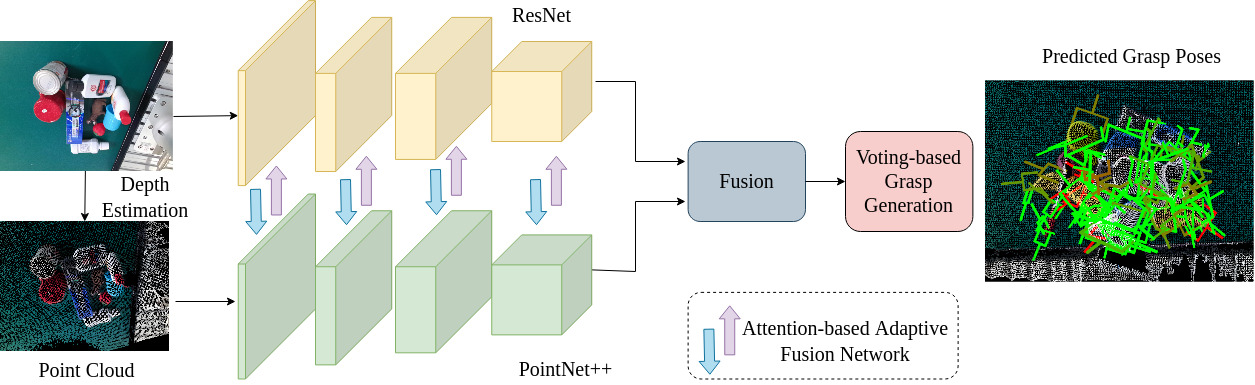
\includegraphics[width=0.98\linewidth]{figs/overview}
	\caption{Overview of our network architecture.}
	\label{fig:Overview}
\end{figure*}
%%%%%%%%%%%%%%%%%%%%%%%%%%%%%%%%%%%%%%%%%%%%%%

\subsection{Depth Estimation}

Existing monocular depth estimation methods are primarily tailored for large outdoor scenes, posing challenges when applied to relatively smaller objects intended for manipulation. To address this limitation, our focus is on enhancing the depth map quality specifically for such objects. We leverage two distinct depth estimation networks, DPT \cite{ranftl2021vision} and iDisc \cite{piccinelli2023idisc}, to derive individual depth images denoted as $\mathbf{I}_{d1}$ and $\mathbf{I}_{d2}$, respectively. By computing the disparity between these images, regions with significant differences beyond a predefined threshold are identified as uncertain areas. Our approach involves excluding these uncertain regions from the depth images and replacing the depth values within other areas with their mean values. This process aims to refine depth information specifically for small object manipulation, culminating in an enhanced and more accurate depth image, denoted as $\mathbf{I}_{d}$.

\subsection{Attention-based Adaptive Fusion Network}

Given a RGB image $\mathbf{I_v}$ and an estimated depth map $\mathbf{I_d}$, our initial step involves elevating the depth image $\mathbf{I_d}$ to a point cloud $\mathbf{P}$ using the camera intrinsic matrix. Subsequently, we employ ResNet34 \cite{he2016deep} and PointNet++ \cite{qi2017pointnet++} to extract visual features $\mathcal{F}_{vis}$ from RGB image and geometric feature $\mathcal{F}_{geo}$ from the point cloud $\mathbf{P}$ respectively. These networks facilitate bidirectional information flow through Visual-Guided Geometric Feature Learning (VGG) and Geometric-Guided Visual Feature Learning (GGV) modules, enabling each branch to utilize mutual local and global information for enhanced representation learning. \\

\textbf{Visual-Guided 3D Geometric Feature Learning}

To integrate visual information from $\mathcal{F}_{vis}^{i}$ into geometric features $\mathcal{F}_{geo}^{i}$ in the $i$-th stage, we introduce a novel Visual-Guided Geometric Feature Learning (VGG) module. Rather than globally compressing the RGB feature map and potentially losing intricate details, we utilize the aligned RGBD image. Each pixel's depth contributes to deriving its corresponding 3D point, establishing an XYZ map aligned with the RGB map. For every geometric feature paired with its 3D point coordinate, we retrieve visual features from $\mathcal{F}_{vis}$ by projecting its neighborhood, with a radius $r_1$, onto the image. Subsequently, we sample the $k_1$ nearest neighbor pixels within this region, gathering their visual features. In cases where fewer than $k_1$ pixels exist in the corresponding region, null features are padded. These collected visual features are integrated using max pooling and processed through Multi-Layer Perceptrons (MLPs) to match their channel size with the point cloud feature. This stage produces modified visual features $\mathcal{F}_{vis}^{'}$. Subsequently, we concatenate the integrated visual features $\mathcal{F}_{vis}^{'}$ with the geometric features $\mathcal{F}_{geo}^{i}$ and apply a shared MLP to obtain the fused geometric feature $\mathcal{F}_{geo}^{fus}$. Consequently, the network enriches $N$ 3D points with high-dimensional features, denoted as $\mathcal{P} = \lbrace p_i \rbrace_{i=1}^{N}$ and $\mathcal{F}_{geo}^{'} = \lbrace f_i \rbrace_{i=1}^{N}$, where $p_i = [ x_i; f_i ]$. Here, $x_i \in \mathbb{R}^{3}$ signifies the point's location in 3D space, and $f_i$ represents the associated feature vector. The enriched points $\lbrace p_{i} \rbrace_{i=1}^{N}$, now imbued with the fused features, are then inputted into our self-attention module to enhance the features $\mathcal{F}_{geo}^{ei}$. In accordance with \cite{zhao2021point, vaswani2017attention}, the self-attention module is defined as follows:


%%%%%%%%%%%%%%%%%%%%%
\begin{equation}
y_{i} = \sum_{p_{j} \in \mathcal{P}(i)} (\alpha(\gamma(p_{i},p_{j}) + \delta) \odot \beta(p_{j}))
\end{equation}
%%%%%%%%%%%%%%%%%%%%%

\noindent $\mathcal{P}(i) \subseteq \mathcal{P}$ refers to a set of points in the local neighborhood of $p_{i}$. $\alpha, \gamma, \delta$, and $\beta$ signify a mapping function, a relation function, a position encoding function, and pointwise feature transformation, respectively. The relation function $\gamma$ uses subtraction to output a vector representing the features of $p_i$ and $p_j$:

%%%%%%%%%%%%%%%%%%%%%
\begin{equation}
\gamma(p_{i},p_{j}) = \varphi(p_i) - \psi(p_j) 
\end{equation}
%%%%%%%%%%%%%%%%%%%%

\noindent Here, $\varphi$ and $\psi$ represent trainable transformations using multilayer perceptrons (MLPs). The mapping function $\alpha$ is an MLP with two linear layers and one ReLU nonlinearity, allowing the module to compute attention weights spatially and across channels while maintaining computational efficiency. To adapt to local data structures, we introduce spatial context using a trainable and parameterized position encoding function $\delta$:

%%%%%%%%%%%%%%%%%%%%%
\begin{equation}
\delta = \phi(x_i - x_j)  
\end{equation}
%%%%%%%%%%%%%%%%%%%%

\noindent $x_i$ and $x_j$ denote the 3D point coordinates for points $i$ and $j$, respectively. The encoding function $\phi$ is an MLP with two linear layers and one ReLU nonlinearity. \\


\textbf{Geometric-Guided Visual Feature Learning}. The Geometric-Guided Visual Feature Learning (GGV) module provides an alternative approach to integrating geometric information from $\mathcal{F}_{geo}^{i}$ into visual features $\mathcal{F}_{vis}^{i}$ during the $i$-th stage. Rather than naively concatenating global point features, this module densely fuses features by identifying $k_{2}$ nearest points for each pixel from the point cloud, collecting corresponding point features, and integrating them via max pooling to produce $\mathcal{F}_{geo}^{'}$. These features are then passed through a spatial attention block $\mathit{M}_{sa1}$ \cite{woo2018cbam}. This mechanism is designed to discern informative regions, eliminating redundant geometric-guided features that may arise from noise or irrelevant areas, thereby facilitating a more effective integration with the visual features $\mathcal{F}_{vis}^{i}$. The block utilizes average-pooling to highlight informative regions, resulting in $\mathcal{F}_{geo}^{avg} \in \mathbb{R}^{W \times H}$. Subsequently, $F_{vis}^{avg}$ undergoes a $7 \times 7$ filter convolution and normalization via the sigmoid function. The output, denoted as $\mathit{M}_{sa1}(\mathcal{F}_{geo}^{i})$, is then element-wise multiplied with the original geometric features, $\mathcal{F}_{geo}^{i}$, to acquire the initial enhanced geometric-guided features, $\mathcal{F}_{geo}^{sa}$. The summarized attention process is illustrated as:

\begin{equation} 
\mathit{M}_{sa1}(\mathcal{F}_{geo}^{i}) = \sigma(f^{7 \times 7}(AvgPool(\mathcal{F}_{geo}^{i})) 
\end{equation}

\begin{equation} 
\mathcal{F}_{geo}^{sa} = \mathit{M}_{sa1}(\mathcal{F}_{geo}^{i}) \otimes \mathcal{F}_{geo}^{i}
\end{equation}

\noindent Here, $\otimes$ denotes element-wise multiplication, $\sigma$ represents the sigmoid function, and $f^{7 \times 7}$ denotes a convolution operation utilizing a $7 \times 7$ filter. Subsequently, $\mathcal{F}_{geo}^{sa}$ is integrated with the visual features $\mathcal{F}_{vis}^{i}$ through element-wise summation to produce the fused features $\mathcal{F}_{vis}^{fus}$:

\begin{equation} 
\mathcal{F}_{vis}^{fus} = \mathcal{F}_{vis}^{i} \oplus \mathcal{F}_{geo}^{sa}
\end{equation}

\noindent Where $\oplus$ signifies element-wise summation. To further refine the fused features $\mathcal{F}_{vis}^{fus}$, a channel attention block $\mathit{M}_{ca}$ \cite{hu2018squeeze} is introduced. This block utilizes global average pooling to reduce each feature map within $\mathcal{F}_{vis}^{fus}$ to a single pixel, generating a 1D vector of length $C$. The vector undergoes an MLP network with a hidden layer and sigmoid activation, followed by element-wise multiplication with $\mathcal{F}_{vis}^{fus}$. This process recalibrates the feature responses, accentuating important channels while suppressing less relevant ones. The output of $\mathit{M}_{ca}$, denoted as $F_{vis}^{c}$, can be summarized as:

\begin{equation} 
\mathit{M}_{ca}(\mathcal{F}_{vis}^{fus}) = \sigma(MLP(AvgPool(\mathcal{F}_{vis}^{fus})) 
\end{equation}

\begin{equation} 
\mathcal{F}_{vis}^{c} = \mathit{M}_{ca}(\mathcal{F}_{vis}^{fus}) \otimes \mathcal{F}_{vis}^{fus}
\end{equation}
 
\noindent Moreover, $\mathcal{F}_{vis}^{c}$ undergoes re-weighting by another spatial attention block, $\mathit{M}_{sa2}$, with components akin to $\mathit{M}_{sa1}$, producing $\mathcal{F}_{vis}^{cs}$. Finally, $\mathcal{F}_{vis}^{cs}$ is integrated with the visual features $\mathcal{F}_{vis}$ through element-wise summation, yielding the enhanced feature representation $\mathcal{F}_{vis}^{ei}$. 

\textbf{Fusion.} Following bidirectional fusion in both VGG and GGV modules, distinct features are extracted by the visual and geometric branches. To generate reliable correspondences and obtain more distinctive features, a simple undirected fusion is performed in the final stage. By projecting each point to the image plane with the camera intrinsic matrix, correspondences between visual and geometry features are established. These pairs are concatenated to form the extracted dense fused feature $\mathcal{F}$, subsequently utilized in the voting-based grasp generation module in the subsequent step.

\subsection{Voting-based Grasp Generation}

Given the extracted dense fused feature $\mathcal{F}=\lbrace{f_i}\rbrace$, we predict grasp poses using the voting-based grasp generation module in our previous work \cite{hoang2023grasp}. Each grasp comprises a center point $p \in \mathbb{R}^3$, a gripper orientation $R \in SO(3)$, a gripper width $w \in \mathbb{R}$, and a grasp score $q \in [0,1]$. We generate $M$ seeds $\lbrace{s_i}\rbrace^{M}_{i=1}$, where each seed $s_i=[x_i,f_i^s]$ holds the 3D spatial location $x_i \in \mathbb{R}^{3}$ and the corresponding feature vector $f_i^s \in \mathbb{R}^{F}$. Processing these seeds through an MLP computes $J$ votes $ \lbrace \lbrace v_{ij}=[y_{ij};f_{ij}^v] \in \mathbb{R}^{3+F} \rbrace_{i=1}^{M} \rbrace_{j=1}^{J}$, leveraging fully connected layers, ReLU activation, and batch normalization. Each vote $v_{ij}$ comprises a 3D point $y_{ij}$ close to a grasp center in Euclidean space and a $F$-dimensional feature vector $f_{ij}^v$. Clustering the votes via uniform sampling and Euclidean distance identifies $K$ votes $\lbrace v_{k}\rbrace_{k=1}^{K}$. Using iterative farthest point sampling (FPS) based on $\lbrace {y_{i}} \rbrace$, $K$ clusters form from the sampled votes, employing a ball query to gather votes within a set radius of the query vote $v_{k}$.

To achieve collision-free grasps in complex environments, comprehending object relationships and contextual cues within features is essential. Our VoteNet integrates a contextual module inspired by self-attention models. It utilizes an MLP and max-pooling to process cluster votes, aggregating into $f_{k}^c \in \mathbb{R}^{F'}$. These vectors compile into a map $f^c = [f_{1}^c; f_{2}^c;...; f_{K}^c ] \in \mathbb{R}^{K \times F'} $, fostering inter-cluster feature communication, significantly enhancing grasp detection performance.

Following the computation of the contextual feature map, our model employs an MLP network to detect a ranked list of grasps $G=(p,R,w,q)$. The prediction layer includes $5+V+2A$ channels: 3 for grasp center regression values, 1 for gripper width regression value, 1 for grasp confidence regression value, $V$ for viewpoint scores, and $A$ each for angle scores and angle residual regression values for in-plane rotation. Here, $V$ and $A$ represent the numbers of sampled viewpoints and in-plane rotations, respectively.

\textbf{Loss Function}: The learning of modules is supervised jointly using a multi-task loss:

\begin{equation}
L_{votegrasp} = \lambda_1 L_{vote} + \lambda_2 L_{grasp}
\label{eq:L_votegrasp_v2}
\end{equation}

The voting loss $L_{vote}$ is a regression loss formulated as:

\begin{equation}
L_{vote} = \frac{1}{M_s} \sum_{i}^{} {\lVert y_i - c^g_i \rVert}_H \cdot \mathds{1}(x_i)
\end{equation}

Here, $M_s$ represents the total number of seed points on the object surface, $c^g_i$ is the closest ground truth grasp center, ${\lVert \cdot \rVert}_H$ denotes the Huber norm, and $\mathds{1}(\cdot)$ is a binary function determining whether a seed point $s_i$ belongs to an object.

The grasp loss function $L_{grasp}$ is defined as:

\begin{equation}
L_{grasp} = L_{center} + \alpha L_{rot} + \beta L_{width} + \gamma L_{score}
\end{equation}

The $L_{grasp}$ comprises losses for grasp center regression ($L_{center}$), rotation ($L_{rot}$), gripper width regression ($L_{width}$), and grasp confidence score regression ($L_{score}$). The grasp center loss includes viewpoint classification loss ($L_{viewpoint}$) and in-plane rotation loss ($L_{in-plane}$), which consists of classification ($L_{angle-cls}$) and regression ($L_{angle-reg}$) losses. Regression losses employ $L1$-smooth loss, while classification losses use standard cross-entropy loss. More details can be found in \cite{hoang2023grasp}.

\subsection{Dataset}

We conduct evaluations and comparisons on the publicly available GraspNet-1Billion dataset \cite{fang2020graspnet}. This dataset comprises 97,280 RGB-D images from 190 cluttered scenes, providing over one billion grasp poses for 88 distinct objects within these scenes. These objects exhibit diversity in shape, texture, size, material, and occlusion conditions, making it an ideal benchmark for assessing our model's generalization capacity and robustness to occlusions. Each object in the dataset is associated with an accurate 3D mesh model, along with camera poses, 6D object poses, object masks, and bounding boxes for all frames. This extensive annotation facilitates straightforward generation of ground truth votes and grasp configurations. Following the methodology of \cite{fang2020graspnet}, we partitioned the dataset into training and testing sets. Specifically, 100 scenes were allocated for training purposes, while 90 scenes were reserved for testing. To evaluate the model's generalizability, the test dataset is further divided into subsets: scenes with novel objects, scenes featuring unseen yet similar objects, and scenes containing previously encountered objects. This deliberate partitioning allows for a comprehensive assessment of our model's performance across diverse scenarios.
